%% Artemis II seismo-acoustic paper -- Seismica submission format
%% Authors: Glenn Thompson (USF), Paul Bremner (NASA MSFC), Han Byul Woo (NASA MSFC), Sue Bilek (NMT) + others
%%
%% Compile from this directory:  ./compile2.sh Artemis2paper.tex
%% Needs seismica.cls, abbrvnat_seismica_upcasetitle.bst and banner.png here.
%% The class loads natbib, hyperref, graphicx, siunitx, amsmath, lineno and
%% xcolor, sets the bibliography style, and (default "review" option) gives
%% one column, double spacing and line numbers.

\documentclass[]{seismica}

%% ---- Extra packages ----
\usepackage{amssymb}
\usepackage{booktabs}        % professional tables
\usepackage{longtable}       % multi-page tables
\usepackage{array}
\usepackage{subcaption}

%% ---- Custom commands ----
\newcommand{\todo}[1]{\textcolor{red}{\textbf{[TODO: #1]}}}
\newcommand{\placeholder}[1]{\textcolor{orange}{\textbf{[#1]}}}

%% ---- Figure path ----
\graphicspath{{figures/}}

%% ---- Title and authors ----
\title{Seismo-acoustic observations of the Artemis~II launch:
  Insights from a dense ground-based network at Kennedy Space Center}
\shorttitle{Seismo-acoustic observations of the Artemis~II launch}

%% TODO: + other authors? Authors or acknowledgements?: Jake Anderson,
%% Pati, Dallin, Erin. Acknowledgements: EPIC, Katherine, Don?, Robert,
%% John?, others?
\author[1]{Glenn Thompson\thanks{Corresponding author: \texttt{thompsong@usf.edu}; ORCID: 0000-0002-9173-0097}}
\author[2]{Paul Bremner}
\author[2]{Han Byul Woo}
\author[3]{Sue Bilek}
\affil[1]{University of South Florida, Tampa, Florida, USA}
\affil[2]{NASA Marshall Space Flight Center, Huntsville, Alabama, USA}
\affil[3]{New Mexico Institute of Mining and Technology, Socorro, New Mexico, USA}

%% ---- Document ----
\begin{document}

\makeseistitle{
  \begin{summary}{Abstract}
  \todo{Write abstract. Key points: dense multi-instrument seismo-acoustic
  network at KSC; Artemis~II (SLS) launch 1~April~2026; infrasound
  amplitude scales with distance, apparent propagation speed $\sim$136~m/s
  (consistent with moving directional source at $\sim$125~m/s in model);
  east--west asymmetry indicates non-isotropic source; seismo-acoustic
  coupling measured at co-located sites.}
  \end{summary}
  %
  \begin{summary}{Non-technical summary}
  \todo{Write non-technical summary (required by Seismica).}
  \end{summary}
}

%% ============================================================
\section{Introduction}

Seismic and infrasound signals generated by rocket launches have been
documented in a number of studies and provide a useful means of
observing energetic, repeatable anthropogenic sources
\citep[e.g.,][]{Kanamori1991,Hupe2019,Pilger2021}.
Launches from Kennedy Space Center and Cape Canaveral Space Force
Station, FL are particularly well suited to such observations due to
their high frequency, diversity of launch vehicles, and accessibility
for ground-based instrumentation.

Since 2016, the University of South Florida (USF) has conducted
intermittent seismic and infrasound monitoring of launches from this
region, resulting in a dataset comprising approximately 140 launches
recorded between 2016 and 2022 \todo{CITE: USF 2016--2022 overview
paper (in preparation; Thompson et al.)\ once available; for now
leave as uncited or note ``Thompson et al., in prep''}. These observations span a wide range of vehicle types and
atmospheric conditions, providing a valuable archive of seismo-acoustic
signals from controlled, high-energy sources. However, the majority of
these launches were recorded by only one to four stations at a time,
limiting the ability to resolve spatial variability in amplitude and
waveform characteristics, as well as source directionality and
propagation effects.

In parallel with these observational efforts, launch activity from
Kennedy Space Center and Cape Canaveral Space Force Station has
increased substantially over the past decade. This increase is driven in
part by the expansion of commercial launch providers, as well as
continued governmental investment in space exploration. The resulting
growth in launch cadence and diversity of vehicle classes---including
the introduction of heavy- and super-heavy-lift systems associated with
the Artemis program---provides new opportunities for detailed
seismo-acoustic observation. Rocket launches constitute repeatable,
high-energy, and well-timed sources, with known origin times and
locations, making them well suited for investigating source radiation
characteristics, propagation through the atmosphere and solid Earth, and
coupling between air pressure and ground motion.

The 2026 Artemis~II launch represents a particularly compelling case
study. As the first crewed mission of the Artemis program, it marks a
major milestone in human spaceflight and is powered by the Space Launch
System (SLS), one of the most energetic launch vehicles ever operated
from this region \citep{NASA_SLS,Sutton2017}. A precursor to this effort, the Artemis~I launch in 2022,
was recorded by a limited network of four stations, demonstrating the
detectability and complexity of the signals generated by the SLS but
also highlighting the limitations imposed by sparse spatial sampling.

In anticipation of Artemis~II, we conducted a dedicated observational
campaign designed to capture a dense, multi-instrument seismo-acoustic
dataset. This deployment combined permanent broadband seismic stations
with temporary nodal seismic arrays and distributed infrasound sensors,
including multiple co-located seismic and infrasound instruments. The
resulting dataset provides substantially improved spatial coverage
compared to previous observations and enables detailed analysis of
amplitude scaling, arrival-time structure, and directional source
effects, as well as direct estimation of seismo-acoustic coupling at
individual sites.

The central premise of this study is that a single, densely instrumented
launch can provide greater insight into source characteristics and
propagation processes than a large number of sparsely recorded events.
We therefore focus on the Artemis~II dataset as a case study to quantify
the dependence of infrasound amplitude and arrival time on distance from
the launchpad, to assess directional asymmetry in the radiated
wavefield, and to estimate frequency-dependent coupling between
atmospheric pressure and ground motion at co-located stations.

While we also consider a simplified forward model of a moving,
directional acoustic source to aid interpretation, the emphasis of this
paper is on direct observational constraints derived from the dense
network. By combining high-quality seismo-acoustic measurements with a
well-characterized, energetic source, this study provides new insight
into the generation and propagation of rocket-induced signals and
establishes a framework for future analyses of both individual launches
and long-term datasets.

The timely nature of this dataset and its relevance to an ongoing
exploration program motivate the rapid presentation of these results.


%% ============================================================
\section{Experiment Design and Instrumentation}

\subsection{Broadband Network Deployment (January 2026)}

A regional broadband seismo-acoustic network was deployed between 7 and
12~January~2026 at Kennedy Space Center. The network consisted of ten
stations, including seven operated by USF and three contributed by NASA
Marshall Space Flight Center (MSFC). All broadband stations remained
operational through the Artemis~II launch on 1~April~2026
(22:35:12~UTC).

The USF stations were equipped with Nanometrics Trillium Compact PH-120
broadband seismometers and Nanometrics Centaur 6-channel digitizers,
recording continuously at 500~Hz. Each USF site included a co-located
infraBSU 0.5-inch microbarometer with a low-frequency corner
near 0.048~Hz and approximately flat response to $\sim$100~Hz
(sensitivity $\sim$\SI{46}{\micro\volt\per\pascal}). One site (B20)
additionally hosted a Chaparral M25 infrasound sensor, providing an
independent measurement of atmospheric pressure over a comparable
frequency band.

The MSFC contribution comprised two broadband stations equipped with
G\"{u}ralp Certimus digital seismometers and one station equipped with a
Silicon Audio accelerometer, also recording at 500~Hz. These stations
extended the spatial coverage of the network and provided complementary
sensor characteristics.

An on-site huddle test was conducted prior to the nodal deployment to
verify instrument performance and network consistency. This test
confirmed timing accuracy, sensor polarity, and overall data quality
across stations, ensuring reliable multi-instrument comparisons.

The co-location of broadband seismic and infrasound sensors at multiple
sites enables direct estimation of frequency-dependent seismo-acoustic
coupling, providing a key observational constraint in this study.

\subsection{Dense Temporary Deployment (March--April 2026)}

A temporary deployment of 33 nodal seismic and infrasound instruments
was carried out on 10--11~March~2026 to support observations of the
Artemis~II launch. These instruments were installed specifically for
this event and were recovered on 3--4~April~2026 following the
successful launch.

The deployment included eleven three-component SmartSolo IGU-16HR-3C
seismic nodes (5~Hz natural frequency) on loan from the EarthScope
Primary Instrument Center (EPIC), and twenty-two Gem infrasound nodes
provided by Boise State University. The Gem infrasound systems have
nominal corner frequencies of approximately 0.039~Hz and 27.1~Hz, with
a sensitivity of $\sim$\SI{3.5}{\milli\pascal\per\text{count}}; after
instrument correction, the usable bandwidth extends approximately from
0.02~Hz to the Nyquist frequency (50~Hz for the 100~Hz sampling rate).

Although a primary goal of the nodal deployment was to enhance spatial
sampling, permitting constraints associated with the Artemis~II mission
limited the installation of new sites. As a result, the nodal
instruments were deployed predominantly at or near existing broadband
stations, forming clusters of co-located sensors rather than expanding
the overall network footprint. Consequently, the principal value of the
nodal deployment lies not in increased spatial coverage, but in improved
calibration and validation of the broadband network.

In particular, the pre-deployment huddle test and subsequent analysis
revealed inconsistencies in amplitude response at several broadband
sites, including signals that were significantly lower than expected and
evidence of at least one malfunctioning broadband sensor. The co-located
nodal instruments therefore provided an essential reference for
assessing data quality, verifying sensor performance, and ensuring that
reliable measurements were obtained at each site during the launch.

A secondary objective of the infrasound deployment was to evaluate
sensor installation methods. At several locations, paired Gem sensors
were deployed both inside existing protective enclosures and in
free-field configurations to assess the influence of enclosure geometry
on recorded signals. This design enables comparison of enclosure effects
on amplitude and spectral content. Channel codes ending in \texttt{HDI}
indicate sensors deployed inside a protective tote enclosure; those
ending in \texttt{HDF} indicate free-field installations without
enclosure.

One broadband site (B05) was not instrumented with nodal equipment due
to access restrictions requiring a security escort, which could not be
arranged during the March deployment period.

The resulting configuration represents a hybrid network in which
permanent broadband stations provide continuous, high-fidelity
recordings, while temporary nodal instruments supply calibration
control, redundancy, and site-specific validation. This combined
approach ensures the reliability of the dataset used in the analyses
presented in this study.

\subsection{Network Geometry}

The spatial distribution of stations relative to the primary launch site
at Space Launch Complex 39B (28.6272$^{\circ}$~N, 80.6208$^{\circ}$~W)
is shown in Figure~\ref{fig:station_map}, and station coordinates are
provided in Table~\ref{tab:stations}. During the Artemis~II launch, the
network spanned source--receiver distances ranging from approximately
0.7~km to 7.6~km.

This geometry provides sensitivity to both radial and azimuthal
variations in the radiated wavefield. Stations located east of the
launchpad sample the downrange portion of the trajectory, while stations
to the west provide complementary coverage of the up-range acoustic
field. The inclusion of multiple co-located instruments at selected
sites further enables assessment of local variability, calibration
consistency, and site-specific seismo-acoustic coupling.

Although not all stations were active simultaneously throughout the
broader deployment period, the configuration during the Artemis~II
launch represents a substantial increase in observational coverage
relative to previous measurements. This dense, partially redundant
network forms the basis for the analyses presented here, including
distance-dependent amplitude scaling, arrival-time structure,
directional asymmetry, and site-specific estimates of seismo-acoustic
coupling.

\begin{table}[htbp]
  \centering
  \caption{Station locations and instrumentation, sorted by distance
    from SLC-39B.}
  \label{tab:stations}
  \small
  \begin{tabular}{lrrrrl}
    \toprule
    Station & Lat ($^{\circ}$) & Lon ($^{\circ}$) & Distance (km) &
      Azimuth ($^{\circ}$) & Instrumentation \\
    \midrule
    B14  & 28.6322 & $-$80.6158 & 0.74 & 41.2  &
      Trillium/Centaur, infraBSU, Gem, SmartSolo \\
    B01  & 28.6214 & $-$80.6067 & 1.53 & 115.1 &
      Trillium/Centaur, infraBSU, Gem, SmartSolo \\
    B03  & 28.6428 & $-$80.6236 & 1.75 & 351.1 &
      Trillium/Centaur, infraBSU, Gem, SmartSolo \\
    B12  & 28.6217 & $-$80.6472 & 2.65 & 256.5 &
      G\"{u}ralp Certimus, Gem, SmartSolo \\
    B05  & 28.6400 & $-$80.6450 & 2.75 & 301.1 &
      Trillium/Centaur, infraBSU \\
    B07  & 28.6072 & $-$80.5942 & 3.42 & 130.5 &
      G\"{u}ralp Certimus, Gem, SmartSolo \\
    B24  & 28.5806 & $-$80.6408 & 5.54 & 200.6 &
      Trillium/Centaur, infraBSU, Gem, SmartSolo \\
    B23  & 28.5786 & $-$80.6078 & 5.55 & 166.7 &
      Silicon Audio accel., Gem, SmartSolo \\
    B24RE& 28.5812 & $-$80.6433 & 5.57 & 203.2 & Gem \\
    B29  & 28.6181 & $-$80.6769 & 5.57 & 259.5 &
      Trillium/Centaur, infraBSU, Gem, SmartSolo \\
    B24LT& 28.5805 & $-$80.6429 & 5.62 & 202.5 & Gem \\
    B20W & 28.5737 & $-$80.5725 & 7.59 & 141.6 & Gem, SmartSolo \\
    B20  & 28.5736 & $-$80.5722 & 7.62 & 141.5 &
      Trillium/Centaur, infraBSU, Chaparral M25, Gem, SmartSolo \\
    B20S & 28.5733 & $-$80.5722 & 7.64 & 141.6 & Gem, SmartSolo \\
    \bottomrule
  \end{tabular}
\end{table}

\begin{figure}[htbp]
  \centering
  %% Source: Box .../writing/Artemis2/artemis2_infrasound_map_abs_peak.pdf
  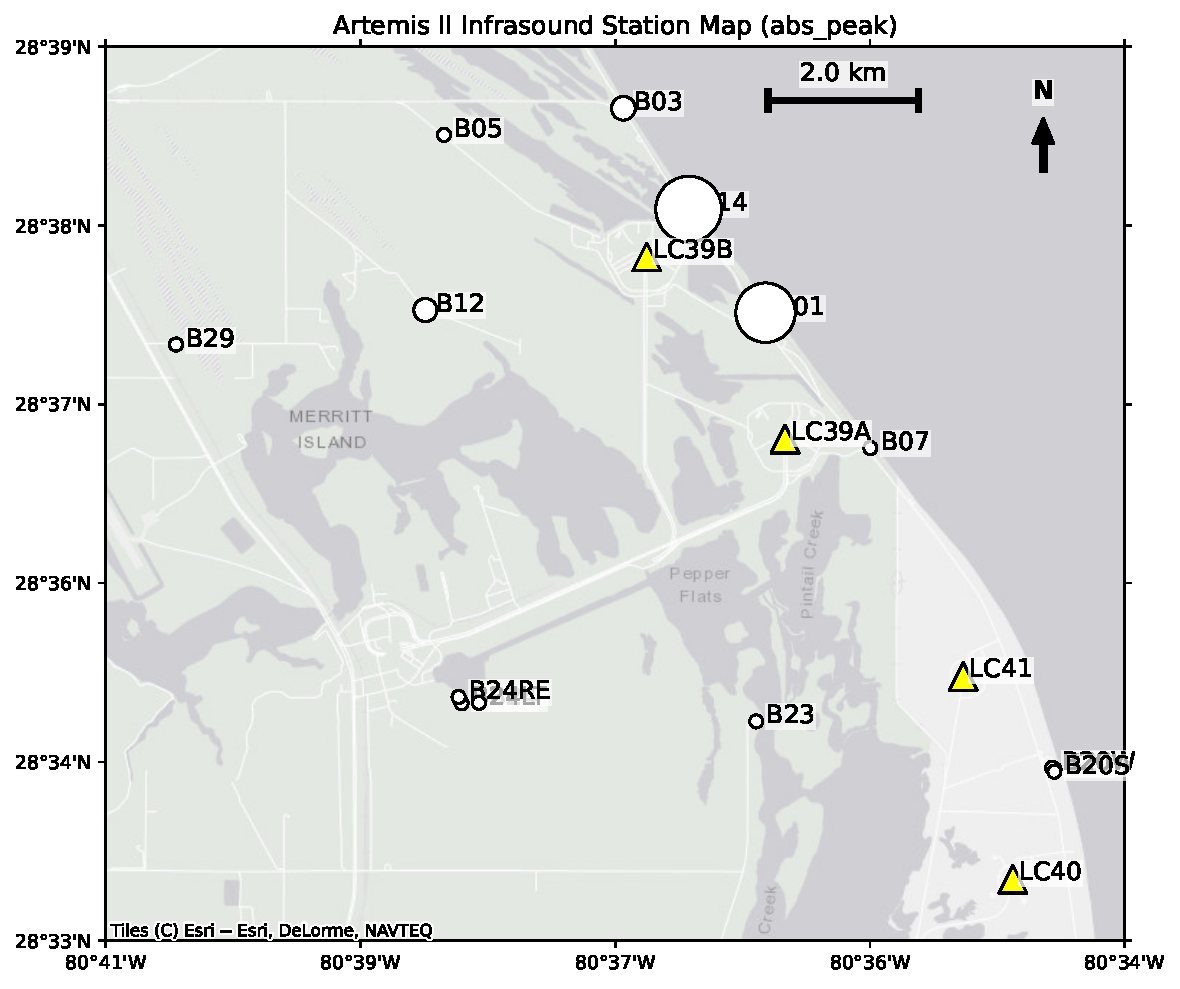
\includegraphics[width=0.95\textwidth]{figures/station_map}
  \caption{Map of infrasound stations (circles) and active launch
    complexes (yellow triangles) for the Artemis~II launch from
    SLC-39B. Station symbols are scaled by peak absolute infrasound
    amplitude.}
  \label{fig:station_map}
\end{figure}


%% ============================================================
\section{Data and Processing}

\subsection{Data Acquisition and Preprocessing}
\label{sec:instruments}

Continuous waveform data were recorded at all stations throughout the
deployment period using a combination of broadband seismic and
infrasound instrumentation (Section~2). Rather than
repeating instrument specifications here, we focus on data retrieval,
preprocessing, and archival procedures used to produce a consistent,
analysis-ready dataset.

At USF broadband sites, Nanometrics Centaur digitizers recorded
continuously to 32--64~GB SD cards using the SeisComP Data Structure
(SDS) format, in which waveform data are organized as daily MiniSEED
files for each SEED identifier. The Silicon Audio accelerometer system
likewise recorded directly to an accessible SD card, producing
one-minute MiniSEED files. In contrast, the G\"{u}ralp Certimus
dataloggers were installed in buried configurations, making physical
access to onboard 128~GB storage impractical during the campaign; only a
targeted time window surrounding the Artemis~II launch was therefore
retrieved via web interface.

The temporary Gem infrasound nodes were recovered following the
deployment and their data converted to MiniSEED using the
\texttt{gemconvert} utility prior to further processing. To ensure
consistency across heterogeneous data sources, all MiniSEED
files---including those from Silicon Audio, Certimus, and Gem
systems---were ingested into a unified SDS archive. The resulting
archive will be deposited with EarthScope to ensure long-term
accessibility and reuse.

\subsection{Signal Preprocessing and Instrument Correction}

Waveform data were processed using the ObsPy framework
\citep{Beyreuther2010} in a standardized workflow
designed to produce consistent, instrument-corrected time series across
all stations.

For each station, waveform segments were extracted from the SDS archive
over a window spanning 30~minutes prior to and 45~minutes following the
Artemis~II launch (22:35:12~UTC on 1~April~2026).

All data were converted to physically meaningful units through
instrument response correction:

\begin{itemize}
  \item \textit{Gem infrasound nodes.}  Corrected to pressure (Pa)
    using the \texttt{gemlog} response functions; effective passband
    $\sim$0.05--50~Hz.
  \item \textit{Nanometrics Trillium Compact seismometers.}  Corrected
    to ground velocity (m~s$^{-1}$) using responses constructed from
    the Nominal Response Library (NRL), specifying the Centaur
    datalogger at 40~V$_\text{pp}$ and the Trillium Compact sensor;
    passband 0.02--235~Hz. A cosine-taper pre-filter of
    (0.01, 0.02, 0.94\,$f_\text{Nyq}$, 0.98\,$f_\text{Nyq}$)~Hz was
    applied.
  \item \textit{infraBSU microbarometers.}  Corrected to pressure (Pa)
    using nominal infraBSU response characteristics at 1~V$_\text{pp}$
    (standard configuration), except at B20 where the DD0 channel
    shares the Centaur Sensor~B input with the Chaparral~M25 and was
    therefore corrected using a 40~V$_\text{pp}$ setting.
  \item \textit{SmartSolo IGU-16HR-3C nodes \citep{SmartSolo2023}.}
    These three-component digital geophone nodes have a natural
    frequency of 5~Hz ($\pm$7.5\%), a damping ratio of $\approx$0.7
    ($\pm$7.5\%), and a geophone sensitivity of approximately
    76.7--80~V~m$^{-1}$~s. The spurious frequency is $>$170~Hz on
    the vertical component. Units were corrected to ground velocity
    (m~s$^{-1}$) using StationXML response files constructed from a
    template response obtained for a representative unit (serial
    number 453013851). Individual station response objects were
    programmatically assigned to each of the 11~units using their
    serial numbers and deployment coordinates. A cosine-taper
    pre-filter of (0.01, 0.02, 0.94\,$f_\text{Nyq}$,
    0.98\,$f_\text{Nyq}$)~Hz was applied.
  \item \textit{G\"{u}ralp Certimus and Silicon Audio systems.}
    Instrument response information was not available at the time of
    analysis; these data were therefore excluded from quantitative
    amplitude comparisons but retained for qualitative assessment.
\end{itemize}

Traces exhibiting effectively constant amplitudes (corresponding to
inactive or unconnected digitizer channels) were identified and removed.
All remaining traces were linearly detrended to remove mean offsets.

\subsection{Amplitude Metrics}

The processed data were trimmed to an analysis window extending from
30~s before to 270~s after the launch time, capturing the primary
acoustic and seismic signals while minimizing contamination from
background noise.

To characterize signal amplitudes in a consistent and robust manner, the
mean was first removed from each trace, and then a sliding 1-second
window analysis was applied to identify the loudest portion of the
signal. The ``peak window'' is defined as the contiguous 1-second
interval whose summed absolute amplitude is largest. Its start time is
recorded as \texttt{peak\_time}.

Amplitude metrics are computed in two ways. The maximum positive
amplitude (\texttt{pos\_max}), maximum negative amplitude
(\texttt{neg\_max}), and maximum absolute amplitude
(\texttt{abs\_peak}) are computed over the entire trimmed trace
(i.e., over the full 300-second analysis window). The median absolute
amplitude (\texttt{median\_abs}), mean absolute amplitude
(\texttt{mean\_abs}), root-mean-square amplitude (\texttt{rms}), and
standard deviation (\texttt{std}) are computed over the peak 1-second
window only. This distinction is preserved in the amplitude tables
below.

For infrasound channels, the RMS amplitude of the peak 1-second window
is converted to sound pressure level (SPL):
\begin{equation}
  L_p = 20\log_{10}\!\left(\frac{p_\mathrm{rms}}{\SI{20}{\micro\pascal}}\right)
  \label{eq:spl}
\end{equation}


%% ============================================================
\section{Observations}
\label{sec:observations}

\subsection{Data Quality and Station Performance}
\label{sec:quality}

The pre-deployment huddle test conducted in January 2026 revealed
amplitude inconsistencies at several broadband sites, motivating the
subsequent temporary nodal deployment as an independent calibration
reference. Analysis of the Artemis~II recordings confirmed these
concerns.

Three broadband stations --- B14, B20, and B24 --- yielded no usable
instrument-corrected seismic recordings despite being nominally
operational through the launch. The cause is not fully resolved; likely
contributors include a defective sensor at one or more sites and
preamplifier issues in the Centaur digitizers identified during the
huddle test. At these stations the co-located Gem infrasound nodes did
record the launch successfully, and those data are included in the
infrasound analysis.

Station B03 recorded the launch seismically, but its amplitudes are
anomalously low by approximately two orders of magnitude relative to
the distance-amplitude trend established by B01, B05, and B29. The
same low-gain signature appears in the B03 infrasound channel
1R.B03.00.DD0 (Table~\ref{tab:infrasound_amplitudes}), which is
consistent with a degraded or low-gain preamplifier in the Centaur
digitizer at B03 affecting all channels on that unit. The 1R.B03.00.DD0
infrasound channel and the B03 seismic channels are excluded from
regression and quantitative amplitude comparisons. The co-located Gem
nodes at B03 (1R.B03..HDI) recorded normally and are retained.

The stations that clearly produced useful broadband seismic recordings
of the Artemis~II launch are B01, B05, and B29. Together with the Gem
infrasound nodes at all sites, these form the primary observational
dataset for the analyses below.

\begin{table}[htbp]
  \centering
  \caption{Infrasound amplitude metrics for all analysed channels during
    the Artemis~II launch, sorted by descending \texttt{abs\_peak}.
    \texttt{peak\_time} (UTC) is the start of the loudest 1-second
    window. \texttt{pos\_max}, \texttt{neg\_max}, and \texttt{abs\_peak}
    are the maximum positive, minimum (most negative), and maximum
    absolute pressure over the entire 300-second analysis window.
    \texttt{median\_abs}, \texttt{mean\_abs}, \texttt{rms}, and
    \texttt{std} are computed within the peak 1-second window only.
    \texttt{spl\_db} is the sound pressure level (dB re
    \SI{20}{\micro\pascal}) derived from the peak-window RMS.
    All pressure values in Pa; SPL in dB.
    Channel codes \texttt{HDI}: sensor inside a protective tote
    enclosure; \texttt{HDF}: free-field installation.}
  \label{tab:infrasound_amplitudes}
  \scriptsize
  \setlength{\tabcolsep}{4pt}
  \begin{tabular}{lrrrrrrrrr}
    \toprule
    \textbf{SEED\_id} & \textbf{peak\_time} & \textbf{pos\_max} &
      \textbf{neg\_max} & \textbf{abs\_peak} & \textbf{median\_abs} &
      \textbf{mean\_abs} & \textbf{rms} & \textbf{std} &
      \textbf{spl\_db} \\
    \midrule
    1R.B14..HDI   & 22:35:27.6 & 569.4  & $-$501.6 & 569.4 & 158.7 & 191.4 & 234.2 & 234.2 & 141.4 \\
    1R.B14..HDF   & 22:35:23.3 & 537.5  & $-$514.3 & 537.5 & 195.0 & 198.0 & 231.3 & 224.1 & 141.3 \\
    1R.B01.00.DD0 & 22:35:33.1 & 507.0  & $-$352.2 & 507.0 & 84.2  & 102.4 & 131.4 & 131.4 & 136.4 \\
    1R.B01..HDI   & 22:35:33.5 & 417.8  & $-$492.1 & 492.1 & 199.2 & 206.2 & 231.0 & 230.8 & 141.3 \\
    1R.B01.00.DD1 & 22:35:33.0 & 475.3  & $-$336.1 & 475.3 & 78.8  & 98.0  & 127.3 & 125.6 & 136.1 \\
    1R.B01.00.DD2 & 22:35:33.6 & 443.4  & $-$330.3 & 443.4 & 79.0  & 95.6  & 121.9 & 121.3 & 135.7 \\
    1R.B05.00.DD0 & 22:35:20.1 & 359.5  & $-$169.4 & 359.5 & 79.8  & 89.0  & 110.6 & 104.4 & 134.9 \\
    1R.B12..HDF   & 22:35:38.6 & 272.7  & $-$293.8 & 293.8 & 93.3  & 100.7 & 118.9 & 118.0 & 135.5 \\
    1R.B03..HDI   & 22:35:34.5 & 210.7  & $-$279.0 & 279.0 & 79.9  & 90.3  & 110.4 & 108.6 & 134.8 \\
    1R.B07.10.HDF & 22:35:47.3 & 166.1  & $-$278.5 & 278.5 & 53.3  & 63.1  & 79.2  & 77.5  & 132.0 \\
    1R.B07..HDF   & 22:35:49.1 & 124.6  & $-$116.1 & 124.6 & 28.0  & 31.9  & 39.7  & 39.7  & 126.0 \\
    1R.B29.00.DD0 & 22:35:52.8 & 108.2  & $-$110.7 & 110.7 & 21.2  & 27.0  & 35.6  & 32.3  & 125.0 \\
    1R.B24LT..HDF & 22:35:48.1 & 108.1  & $-$75.0  & 108.1 & 17.6  & 23.1  & 28.2  & 28.2  & 123.0 \\
    1R.B29..HDF   & 22:35:52.8 & 103.2  & $-$82.0  & 103.2 & 22.6  & 26.6  & 32.5  & 32.5  & 124.2 \\
    1R.B24RE..HDF & 22:35:48.9 & 100.8  & $-$67.9  & 100.8 & 19.6  & 21.5  & 25.7  & 25.7  & 122.2 \\
    1R.B29..HDI   & 22:35:52.8 & 96.9   & $-$89.0  & 96.9  & 20.1  & 24.9  & 31.1  & 31.1  & 123.8 \\
    1R.B23..HDF   & 22:35:57.7 & 83.4   & $-$62.1  & 83.4  & 17.8  & 23.5  & 30.5  & 30.5  & 123.7 \\
    1R.B24..HDF   & 22:35:51.1 & 82.5   & $-$62.2  & 82.5  & 17.4  & 21.1  & 25.7  & 25.7  & 122.2 \\
    1R.B20..HDF   & 22:36:25.2 & 45.1   & $-$40.6  & 45.1  & 10.4  & 12.4  & 15.5  & 15.4  & 117.8 \\
    1R.B20W..HDF  & 22:36:08.2 & 44.6   & $-$36.4  & 44.6  & 11.0  & 12.5  & 14.9  & 14.9  & 117.5 \\
    1R.B20.10.HDI & 22:36:25.0 & 42.4   & $-$43.3  & 43.3  & 10.1  & 12.4  & 15.4  & 15.4  & 117.7 \\
    1R.B20S..HDF  & 22:36:25.9 & 41.7   & $-$38.2  & 41.7  & 10.0  & 11.4  & 14.4  & 14.3  & 117.1 \\
    1R.B03.00.DD0$^{\dagger}$ & 22:35:17.0 & 0.3 & $-$0.6 & 0.6 & 0.1 & 0.2 & 0.2 & 0.2 & 80.7 \\
    \bottomrule
    \multicolumn{10}{l}{$^{\dagger}$ Anomalously low; excluded from
      quantitative analyses. See Section~\ref{sec:quality}.}
  \end{tabular}
\end{table}

\begin{table}[htbp]
  \centering
  \caption{Seismic amplitude metrics for all analysed channels during
    the Artemis~II launch, sorted by descending \texttt{abs\_peak}.
    Column definitions as in Table~\ref{tab:infrasound_amplitudes}
    except all values are ground velocity (m~s$^{-1}$) and there is no
    SPL column. Only stations that yielded usable instrument-corrected
    seismic recordings are included. Broadband stations B14, B20, and
    B24 produced no usable seismic result despite being nominally
    operational (see Section~\ref{sec:quality}); B03 recorded the
    launch but at anomalously low amplitude, consistent with a
    degraded Centaur preamplifier gain (also flagged in
    Table~\ref{tab:infrasound_amplitudes}).}
  \label{tab:seismic_amplitudes}
  \scriptsize
  \setlength{\tabcolsep}{4pt}
  \begin{tabular}{lrrrrrrrr}
    \toprule
    \textbf{SEED\_id} & \textbf{peak\_time} & \textbf{pos\_max} &
      \textbf{neg\_max} & \textbf{abs\_peak} & \textbf{median\_abs} &
      \textbf{mean\_abs} & \textbf{rms} & \textbf{std} \\
    \midrule
    1R.B01.00.DHZ & 22:35:37.2 & $2.62\times10^{-3}$ & $-2.91\times10^{-3}$ & $2.91\times10^{-3}$ & $6.91\times10^{-4}$ & $7.47\times10^{-4}$ & $9.18\times10^{-4}$ & $9.16\times10^{-4}$ \\
    1R.B01.00.DH2 & 22:35:33.9 & $1.85\times10^{-3}$ & $-2.20\times10^{-3}$ & $2.20\times10^{-3}$ & $5.89\times10^{-4}$ & $6.43\times10^{-4}$ & $7.74\times10^{-4}$ & $7.72\times10^{-4}$ \\
    1R.B01.00.DH1 & 22:35:30.2 & $1.80\times10^{-3}$ & $-2.04\times10^{-3}$ & $2.04\times10^{-3}$ & $5.16\times10^{-4}$ & $5.74\times10^{-4}$ & $6.78\times10^{-4}$ & $6.74\times10^{-4}$ \\
    1R.B05.00.DHZ & 22:35:21.2 & $1.70\times10^{-3}$ & $-7.52\times10^{-4}$ & $1.70\times10^{-3}$ & $2.33\times10^{-4}$ & $2.45\times10^{-4}$ & $2.86\times10^{-4}$ & $2.86\times10^{-4}$ \\
    1R.B29.00.DH2 & 22:35:53.4 & $1.29\times10^{-3}$ & $-1.21\times10^{-3}$ & $1.29\times10^{-3}$ & $3.66\times10^{-4}$ & $4.00\times10^{-4}$ & $4.77\times10^{-4}$ & $4.77\times10^{-4}$ \\
    1R.B29.00.DHZ & 22:35:53.3 & $9.79\times10^{-4}$ & $-8.47\times10^{-4}$ & $9.79\times10^{-4}$ & $2.70\times10^{-4}$ & $2.91\times10^{-4}$ & $3.52\times10^{-4}$ & $3.52\times10^{-4}$ \\
    1R.B05.00.DH1 & 22:35:21.2 & $9.18\times10^{-4}$ & $-8.63\times10^{-4}$ & $9.18\times10^{-4}$ & $2.83\times10^{-4}$ & $2.98\times10^{-4}$ & $3.47\times10^{-4}$ & $3.47\times10^{-4}$ \\
    1R.B29.00.DH1 & 22:35:53.3 & $6.66\times10^{-4}$ & $-6.57\times10^{-4}$ & $6.66\times10^{-4}$ & $1.84\times10^{-4}$ & $1.98\times10^{-4}$ & $2.40\times10^{-4}$ & $2.40\times10^{-4}$ \\
    1R.B03.00.DH1 & 22:35:32.0 & $7.27\times10^{-5}$ & $-4.43\times10^{-5}$ & $7.27\times10^{-5}$ & $6.18\times10^{-6}$ & $9.03\times10^{-6}$ & $1.32\times10^{-5}$ & $1.32\times10^{-5}$ \\
    1R.B03.00.DHZ & 22:35:34.3 & $6.62\times10^{-5}$ & $-7.17\times10^{-5}$ & $7.17\times10^{-5}$ & $5.74\times10^{-6}$ & $9.90\times10^{-6}$ & $1.45\times10^{-5}$ & $1.45\times10^{-5}$ \\
    1R.B05.00.DH2 & 22:35:34.9 & $3.53\times10^{-5}$ & $-2.32\times10^{-5}$ & $3.53\times10^{-5}$ & $4.04\times10^{-6}$ & $5.43\times10^{-6}$ & $7.35\times10^{-6}$ & $7.05\times10^{-6}$ \\
    1R.B03.00.DH2 & 22:35:34.3 & $1.96\times10^{-5}$ & $-1.68\times10^{-5}$ & $1.96\times10^{-5}$ & $1.88\times10^{-6}$ & $2.68\times10^{-6}$ & $3.78\times10^{-6}$ & $3.78\times10^{-6}$ \\
    \bottomrule
  \end{tabular}
\end{table}

\subsection{Amplitude versus Distance}

\begin{figure}[htbp]
  \centering
  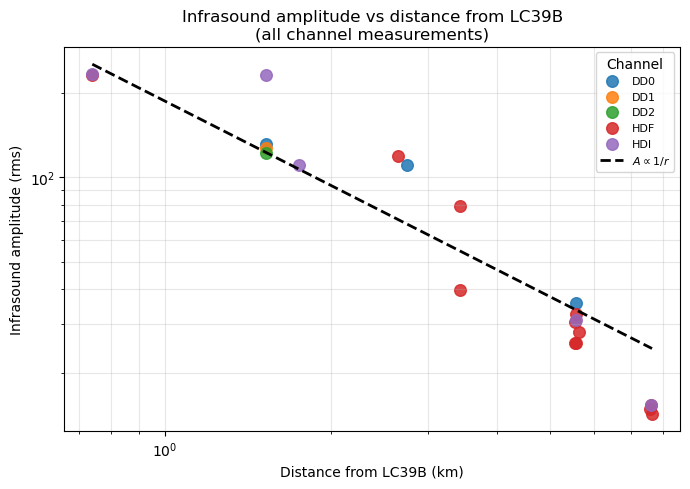
\includegraphics[width=\textwidth]{figures/infrasound_amplitude_vs_distance}
  \caption{Peak infrasound RMS amplitude (Pa) versus sensor distance
    from SLC-39B. Each point represents one SEED channel, coloured by
    channel type: DD0/1/2 (infraBSU), HDF (Gem free-field), HDI (Gem
    inside tote enclosure). The dashed line shows a reference $A
    \propto 1/R$ curve fitted to the data. The best-fit power law
    (Equation~\ref{eq:amplitude_decay}) has a steeper decay exponent
    of $-1.22$. Channel 1R.B03.00.DD0 (anomalously low; Centaur
    preamplifier failure) is excluded.}
  \label{fig:amplitude_distance}
\end{figure}

The best-fit power-law relationship between peak RMS infrasound
amplitude $A_\text{RMS}$ and source--receiver distance $R$ is:
\begin{equation}
  \log_{10}(A_\text{RMS}) = 2.36 - 1.22\,\log_{10}(R)
  \label{eq:amplitude_decay}
\end{equation}
where $R$ is in km. The exponent of $-1.22$ implies somewhat faster
decay than the $1/R$ expected for a stationary, isotropic point source
(exponent $-1.0$). This is consistent with an accelerating, anisotropic
source moving away from the network.

\subsection{Peak Arrival Time versus Distance}

\begin{figure}[htbp]
  \centering
  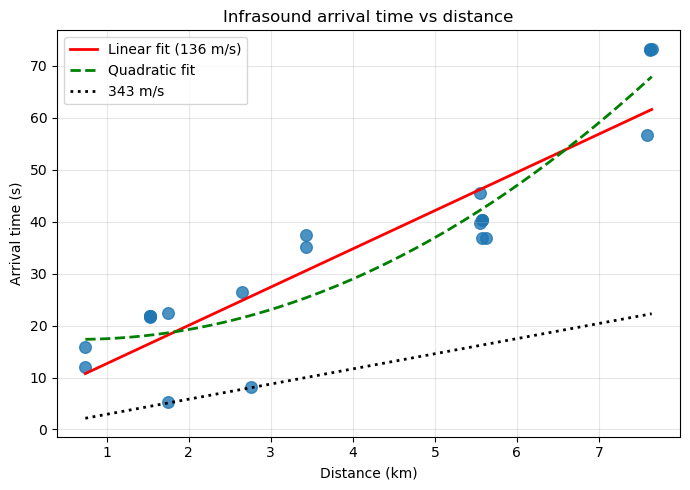
\includegraphics[width=\textwidth]{figures/infrasound_arrival_time_vs_distance}
  \caption{Peak infrasound arrival time (s after launch) versus
    station distance from SLC-39B (km). The solid red line shows the
    best linear fit ($t = 5.31 + 7.37\times10^{-3}\,r$, $r$ in~m;
    apparent speed 136~m~s$^{-1}$); the dashed green line shows the
    quadratic fit; the dotted black line shows the expected travel time
    at the ambient sound speed (343~m~s$^{-1}$) for reference.
    The much lower apparent speed reflects source motion and the fact
    that the dominant signal arrives from a point along the ascent
    trajectory rather than from the launchpad itself.}
  \label{fig:arrival_time}
\end{figure}

The observed arrival times do not conform to propagation at the ambient
sound speed (343~m~s$^{-1}$). The best-fit linear and quadratic
relationships are:
\begin{align}
  t &= 5.3 + 7.4\,R \label{eq:tlin} \\
  t &= 17.8 - 1.3\,R + 0.001\,R^2 \label{eq:tquad}
\end{align}
where $t$ is in seconds and $R$ is in km. The linear fit yields an
apparent propagation speed of approximately 136~m~s$^{-1}$, well below
the speed of sound. This apparent slowness reflects the geometry of a
moving, elevated source: the dominant signal arrives not from the pad
but from a point along the trajectory at some time after launch.

\subsection{Outliers and Variability}

\todo{Identify anomalous channels; discuss possible causes: instrument
issues (B03), local site effects, directionality.}

\subsection{East--West Asymmetry}

\todo{Compare east (downrange) vs.\ west (uprange) stations in
amplitude and timing. Early indication of non-isotropic source.}


%% ============================================================
\section{Anatomy of a Rocket Seismogram}

\begin{figure}[htbp]
  \centering
  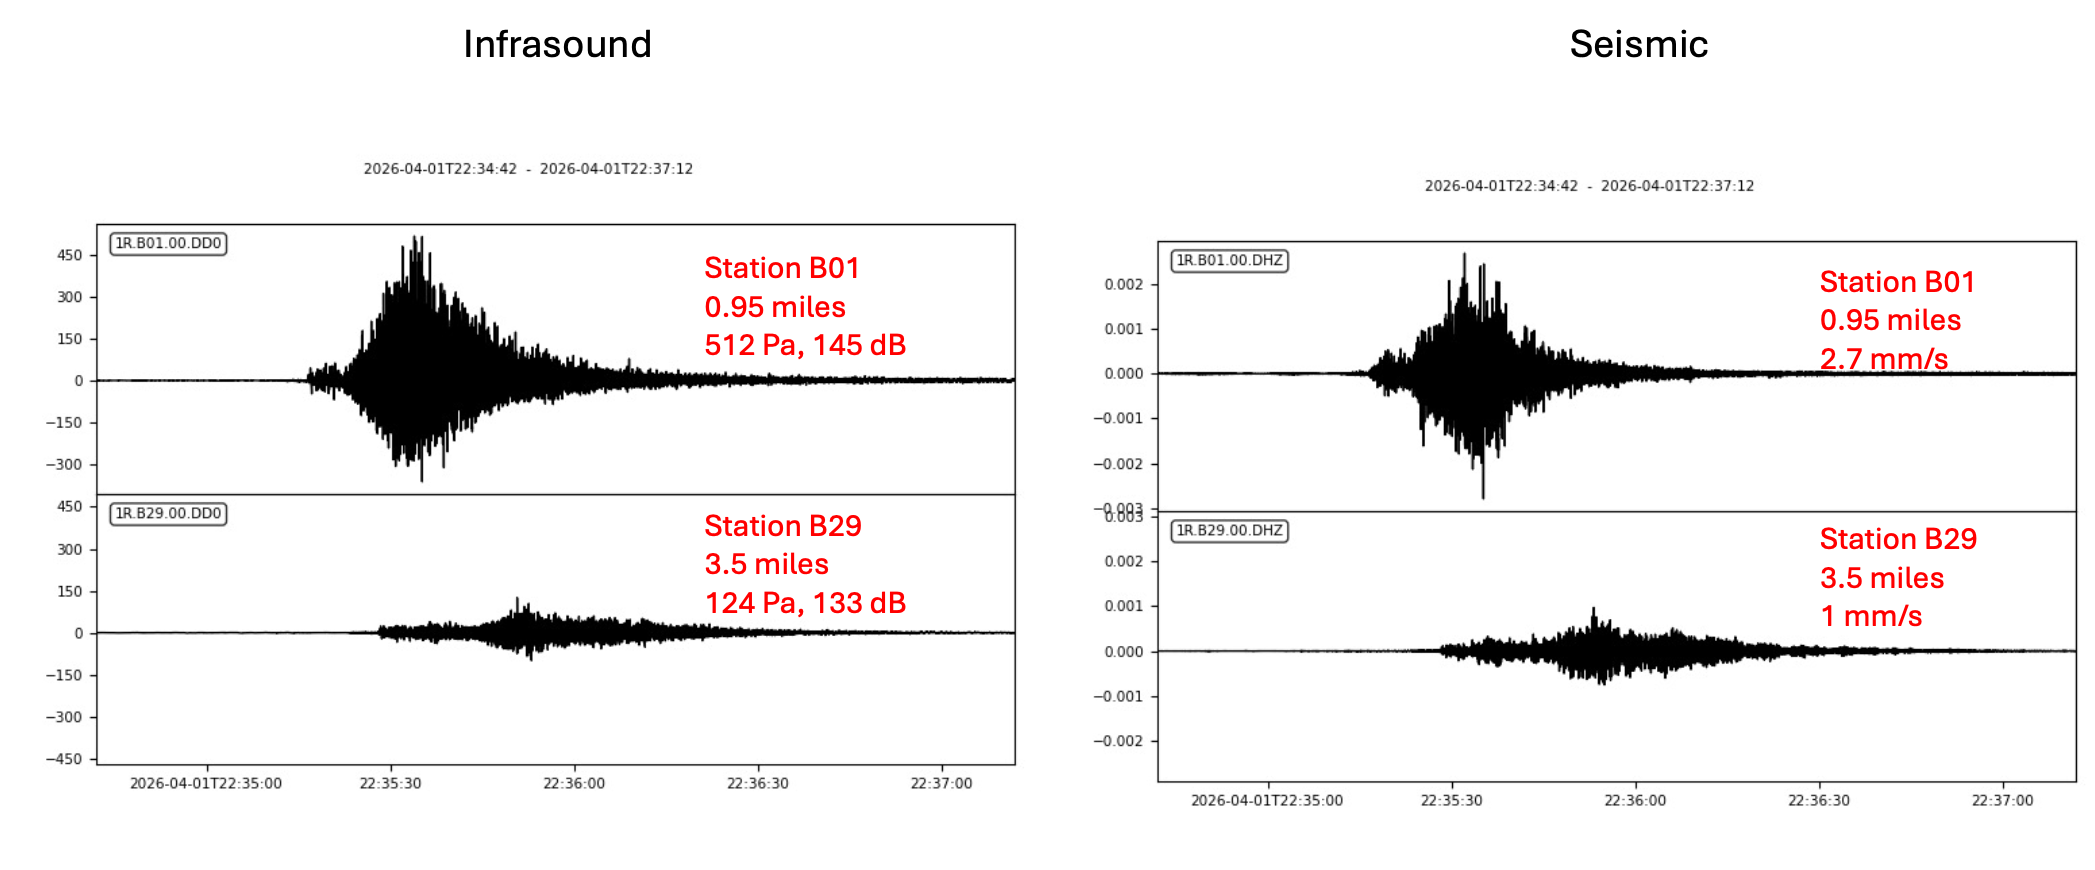
\includegraphics[width=\textwidth]{figures/near_far_waveforms}
  \caption{Infrasound (left) and seismic vertical (right) waveforms
    recorded at stations B01 (1.53~km from SLC-39B; peak 507~Pa,
    145~dB) and B29 (5.57~km; peak 111~Pa, 125~dB) during the
    Artemis~II launch on 1~April~2026. Time window: 22:34:42--22:37:12
    UTC. The signal onset at B01 arrives approximately 11~s after
    launch; the more distant B29 shows a later, lower-amplitude arrival
    with a broader envelope.}
  \label{fig:waveforms}
\end{figure}

\begin{figure}[htbp]
  \centering
  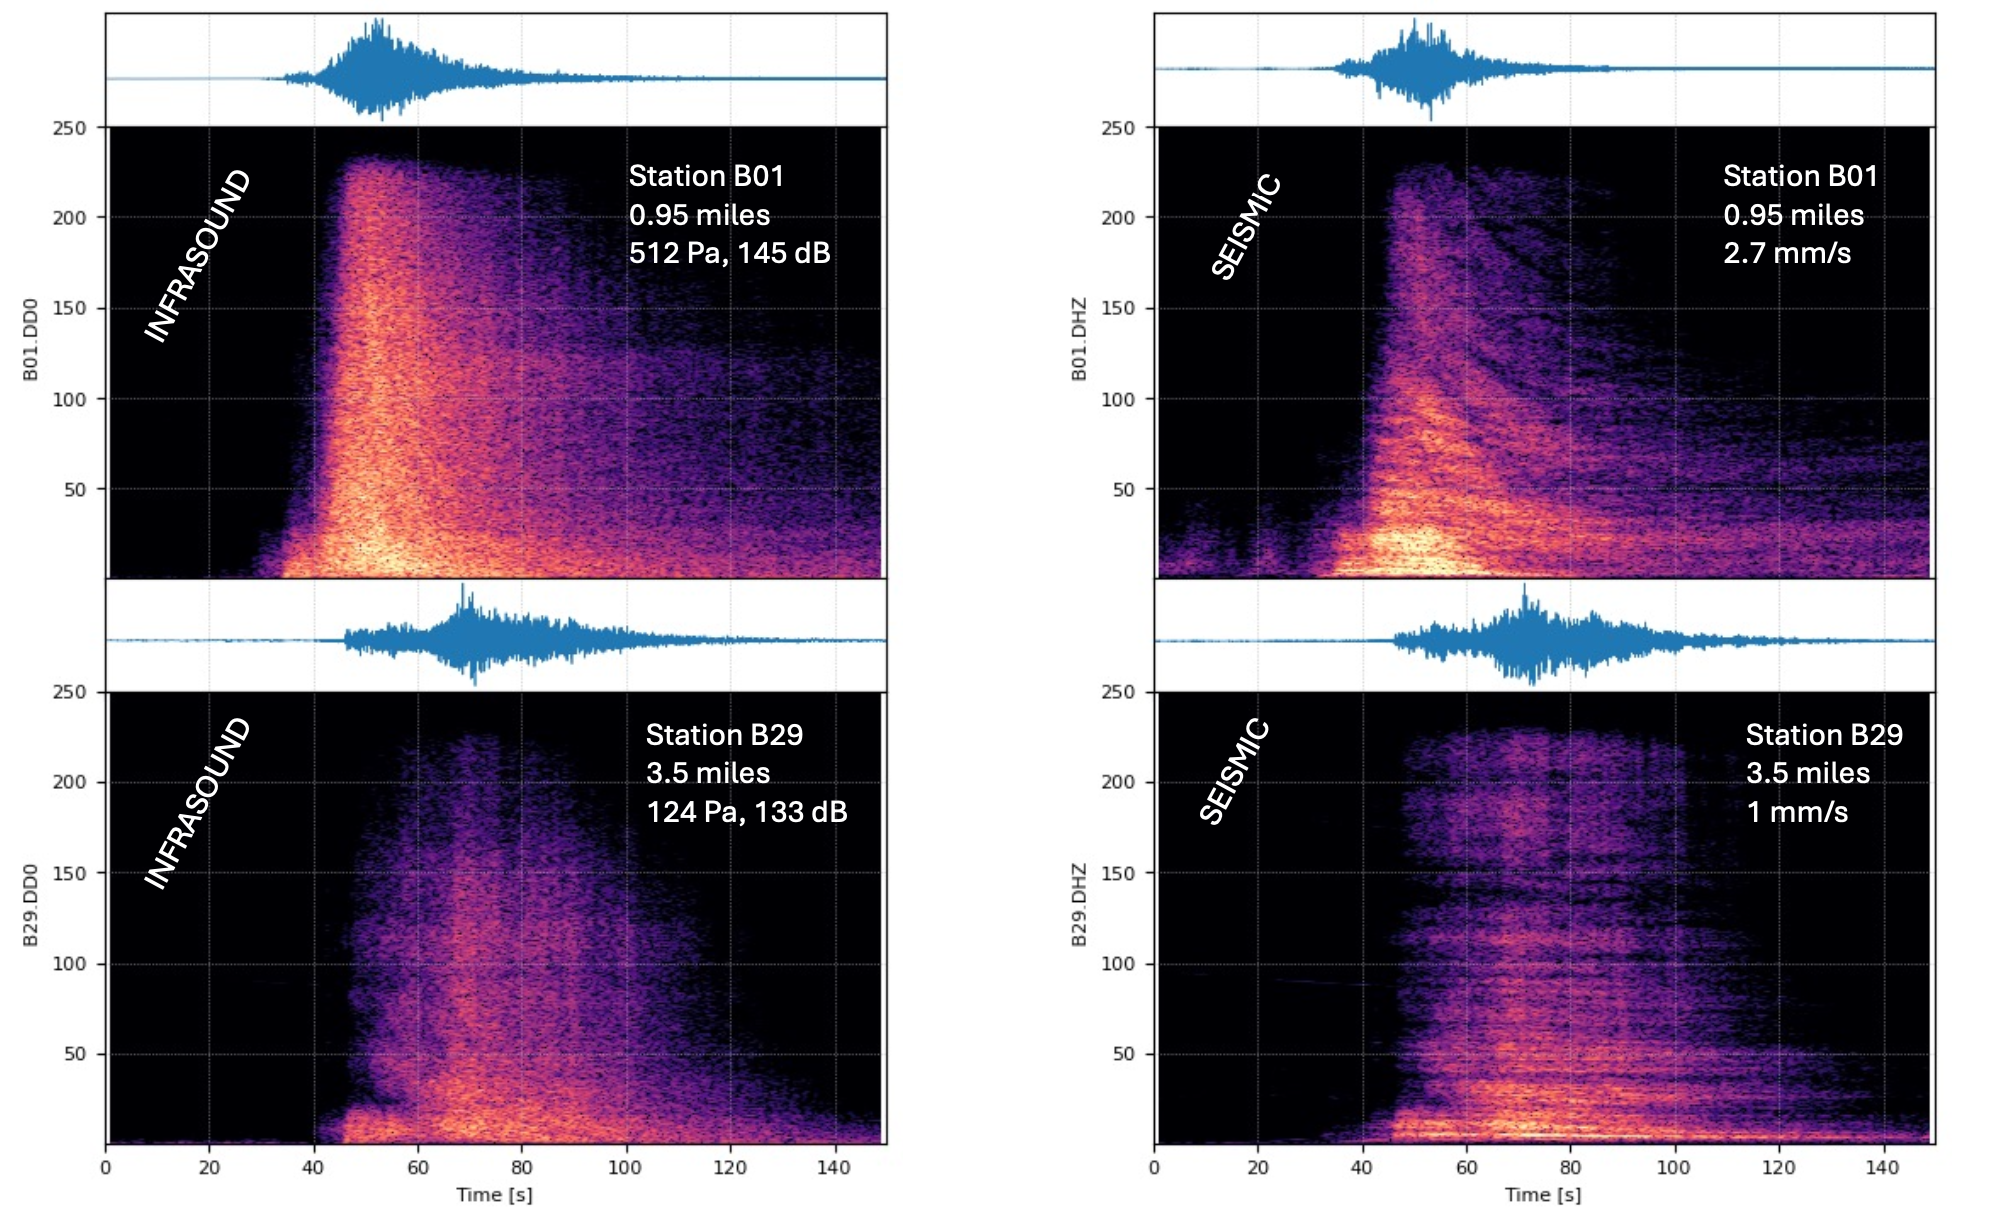
\includegraphics[width=\textwidth]{figures/near_far_spectrograms}
  \caption{Infrasound (left columns) and seismic vertical (right
    columns) spectrograms at stations B01 (top panels) and B29 (bottom
    panels) during the Artemis~II launch. Time is seconds after
    22:34:00~UTC. Broadband energy extends to $>$250~Hz. The
    high-amplitude broadband onset, coinciding with the main acoustic
    arrival, is followed by a gradual frequency roll-off as the rocket
    ascends and the source moves away from the network.}
  \label{fig:spectrograms}
\end{figure}

\todo{Write prose for this section.}


%% ============================================================
\section{Infrasound-to-Seismic Coupling}

\todo{Add spectral ratio plots of seismic to infrasound data, yielding
coupling coefficients as a function of frequency in
m~s$^{-1}$~Pa$^{-1}$. Consider comparing velocity and acceleration
seismograms (pressure = force/area; acceleration = force/mass).}


%% ============================================================
\section{Forward Modeling}
\label{sec:modeling}

\subsection{Model Overview}

To aid interpretation of the observed seismo-acoustic signals, we
implement a simplified forward model representing the rocket as a
moving, time-dependent acoustic source. The model is designed to capture
first-order effects associated with source motion, directional
radiation, and geometric spreading, while remaining computationally
efficient and consistent with the available observational constraints.

The rocket trajectory is represented using an idealized gravity-turn
formulation in which the vehicle initially ascends vertically before
progressively pitching over into a downrange trajectory. Acoustic
propagation from the source to each station is modeled assuming a
constant sound speed, neglecting atmospheric stratification and wind
effects. While this assumption limits accuracy at longer ranges, it
provides a useful baseline for interpreting apparent propagation
velocities derived from the data.

The acoustic source is modeled as a point source with directional
radiation described by a conical emission pattern, capturing the strong
anisotropy associated with rocket exhaust noise. As an extension, the
framework also allows for a distributed source representation along the
exhaust plume, although this is not required for the primary comparisons
presented here.

\subsection{Rocket Trajectory Model}

The rocket trajectory is parameterized in terms of time-dependent
position, velocity, and orientation, following a simplified gravity-turn
model. The trajectory is divided into three phases: an initial vertical
ascent, a controlled pitchover maneuver, and a gravity-driven turn.

Model parameters were selected to approximate the early flight profile
of the Artemis~II launch. The nominal thrust is 37.4~MN (corresponding
to 8.4~million~lbf average over the first two minutes), with a simple
throttle schedule applied: full thrust for the first 60~s, reduced to
88\% between 60--80~s, then 95\% between 80--128~s. The initial vehicle
mass is $2.61\times10^{6}$~kg, with a constant mass depletion rate of
\SI{12081}{\kilo\gram\per\second}, representing propellant consumption
by the core stage and solid rocket boosters. Gravitational acceleration
is fixed at \SI{9.81}{\metre\per\second\squared}.

The pitch program is defined by three parameters: an initial vertical
ascent of 6~s, a brief 2$^{\circ}$ pitchover beginning at 10~s, and a
constant pitch rate of 0.45$^{\circ}$~s$^{-1}$ thereafter up to a
maximum pitch angle of 80$^{\circ}$.

Aerodynamic drag is included using a Mach-dependent drag coefficient
(subsonic $C_D \approx 0.30$, rising to 0.60 at transonic, declining to
0.35 at supersonic), with a reference area of 78~m$^2$ and an
exponentially decreasing atmospheric density profile (sea-level density
1.225~kg~m$^{-3}$, scale height 8.5~km). The local sound speed for
Mach number calculation uses a tropospheric temperature lapse rate of
6.5~K~km$^{-1}$, constant below 11~km.

\subsection{Acoustic Source Model}

The acoustic source is modeled as a time-dependent emitter whose
amplitude and directivity vary with source strength and geometry. The
amplitude observed at a station is:
\begin{equation}
  A(t) \propto \frac{Q(t)\,D(\phi)}{R(t)}
  \label{eq:source}
\end{equation}
where $Q(t)$ is the source strength, $D(\phi)$ is a directional
radiation function, and $R(t)$ is the instantaneous source--receiver
distance. The angle $\phi$ is measured between the exhaust direction
(anti-parallel to the velocity vector) and the direction from the
source to the receiver. Directional radiation is represented by a
Gaussian cone model:
\begin{equation}
  D(\phi) = \exp\!\left[-\frac{1}{2}\left(\frac{\phi - \phi_0}{\sigma}\right)^2\right]
  \label{eq:directivity}
\end{equation}
in which acoustic energy is preferentially emitted at angle $\phi_0$
relative to the exhaust axis, with angular width $\sigma$. The source
strength $Q(t)$ rises from zero following launch with a time constant
$\tau_\mathrm{rise} = 8$~s, reflecting the ramp-up of engine noise.

\subsection{Trajectory Validation}

\begin{figure}[htbp]
  \centering
  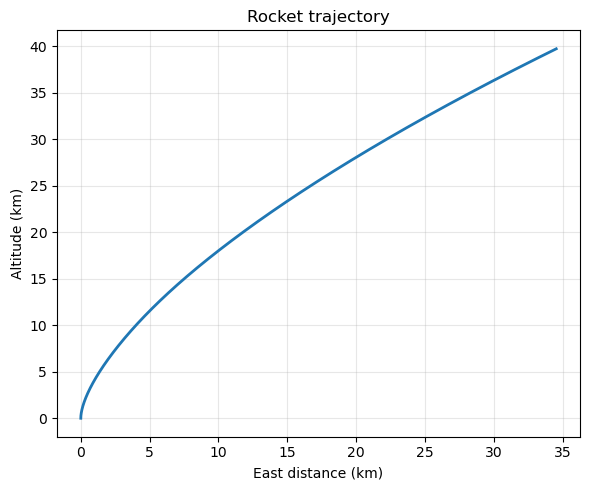
\includegraphics[width=0.8\textwidth]{figures/trajectory}
  \caption{Modeled rocket trajectory during the first 120~s of flight,
    showing altitude as a function of downrange distance.}
  \label{fig:trajectory}
\end{figure}

\begin{figure}[htbp]
  \centering
  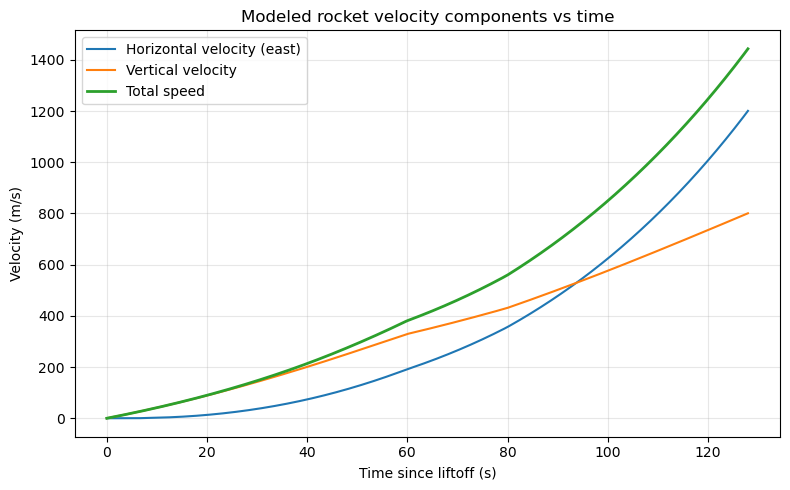
\includegraphics[width=0.85\textwidth]{figures/velocity_vs_time}
  \caption{Modeled rocket velocity components and total speed versus
    time since liftoff. The rocket transitions from predominantly
    vertical (orange) to predominantly horizontal (blue) motion around
    T+90~s, with total speed (green) reaching $\sim$1\,440~m~s$^{-1}$
    at T+128~s, consistent with solid rocket booster separation.}
  \label{fig:speed}
\end{figure}

The simulated trajectory reproduces the expected qualitative features of
a gravity-turn ascent: an initial near-vertical rise followed by a
gradual transition to downrange motion. Quantitatively, the model
reproduces (i)~transonic conditions at approximately 60--70~s,
(ii)~rapid acceleration through the lower atmosphere, and
(iii)~altitudes of order 40--50~km by approximately 120~s. This level
of agreement is sufficient for the purposes of the forward model, which
is intended to reproduce relative variations in arrival time and
amplitude as a function of station geometry.

\subsection{Synthetic Predictions}

To isolate the effect of source motion and directivity from
site-specific complications, we computed synthetic infrasound envelopes
along two idealized station lines extending due east (downrange) and
due west (uprange) of SLC-39B, at 0.5~km spacing out to 16~km
(64~virtual stations in total). Each point on the modeled trajectory,
emitted at source time $t_s$, contributes an amplitude given by
Equation~\ref{eq:source} at observed time $t_s + R/c$, where
$c = 343$~m~s$^{-1}$ is the ambient sound speed; the synthetic envelope
is this amplitude as a function of observed time. Because $Q(t)$ is not calibrated in
absolute units, synthetic amplitudes are normalized and only their
relative variation with distance and azimuth is interpreted.

Figure~\ref{fig:synthetic_envelopes} shows envelopes at 1, 4, and 8~km
on each line. At all distances the peak is broad (tens of seconds) and
arrives well after the direct travel time from the pad, because the
dominant contribution comes from a point on the ascent trajectory where
the receiver lies within the directivity lobe. The model predicts a
strong east--west asymmetry. West stations peak earlier and louder than
east stations at the same distance: the delay grows from 5~s at 1~km
to 35~s at 8~km, and the west/east amplitude ratio grows from 1.2 to
1.45. This follows from the geometry of an aft-directed lobe on a
downrange trajectory. West stations lie behind the rocket from the
start and are illuminated early in the flight (source times of
22--48~s for stations at 1--8~km). East stations are crossed by the
lobe only after the rocket has climbed and moved downrange of them
(source times of 27--74~s), so the sound travels further and arrives
later. The angle $\phi$ at the time of peak contribution is nearly
constant along each line ($35$--$37^\circ$ west, $39$--$42^\circ$ east),
confirming that the peak is controlled by the directivity function
rather than by the minimum source--receiver distance.

Synthetic peak amplitude decays with distance as a power law with
exponent $-0.96$ for both lines combined ($-0.92$ west, $-1.00$ east;
Figure~\ref{fig:synthetic_amplitude}), close to the $1/R$ term in
Equation~\ref{eq:source}. This is shallower than the observed exponent
of $-1.22$ (Equation~\ref{eq:amplitude_decay}), indicating that the
current model omits a distance-dependent loss mechanism such as
atmospheric absorption, ground interaction or refraction.

Synthetic peak arrival time increases approximately linearly with
distance (Figure~\ref{fig:synthetics}). A single linear fit to both
lines gives

\begin{figure}[htbp]
  \centering
  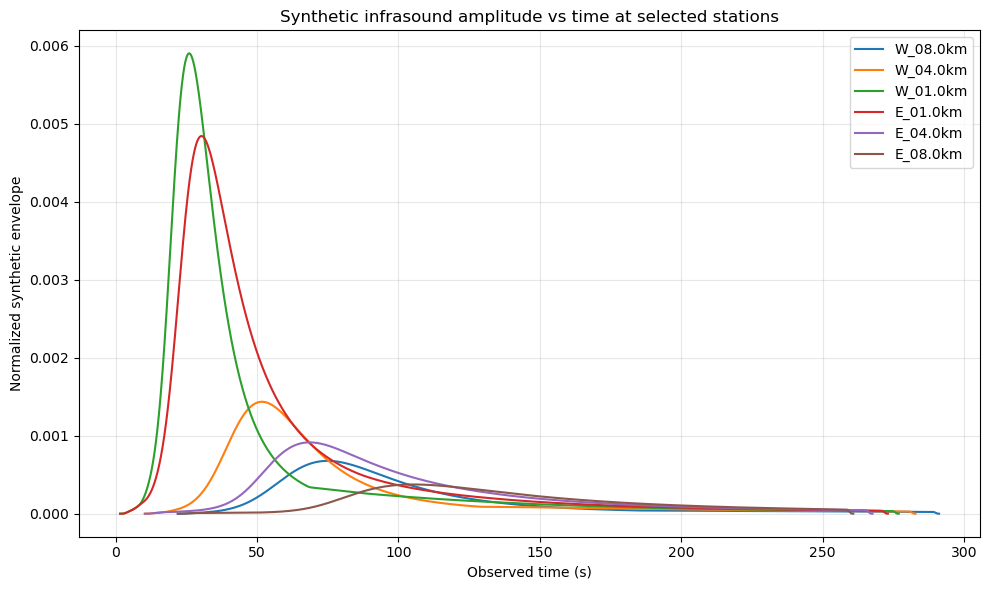
\includegraphics[width=\textwidth]{figures/synthetic_envelopes}
  \caption{Synthetic infrasound amplitude envelopes at selected west
    (W) and east (E) stations as a function of observed time (s after
    launch). Closer stations show earlier, sharper peaks. At a given
    distance, west stations peak earlier and with higher amplitude
    than east stations, reflecting the aft-directed source on a
    downrange trajectory.}
  \label{fig:synthetic_envelopes}
\end{figure}

\begin{figure}[htbp]
  \centering
  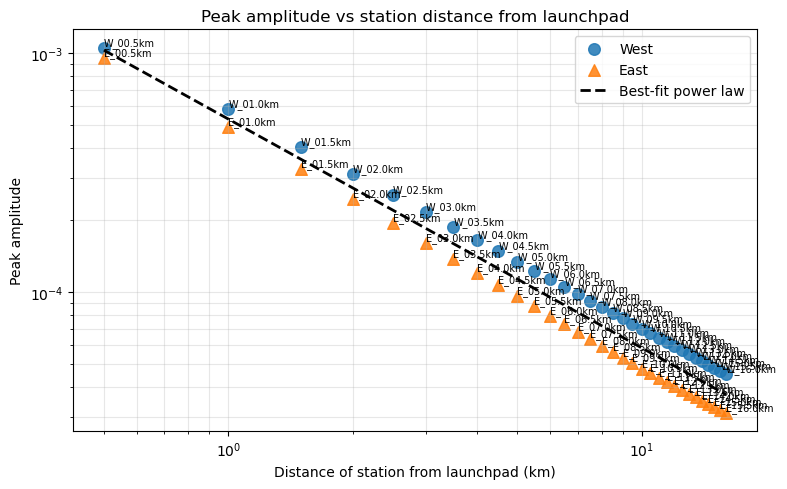
\includegraphics[width=\textwidth]{figures/synthetic_amplitude_vs_distance}
  \caption{Synthetic peak amplitude versus station distance from
    SLC-39B for west (circles) and east (triangles) stations. The
    dashed line shows the best-fit power-law decay (exponent $-0.96$).
    West (uprange) stations consistently show higher amplitudes than
    east (downrange) stations at the same distance, reflecting the
    aft-directed directivity of the acoustic source.}
  \label{fig:synthetic_amplitude}
\end{figure}

\begin{figure}[htbp]
  \centering
  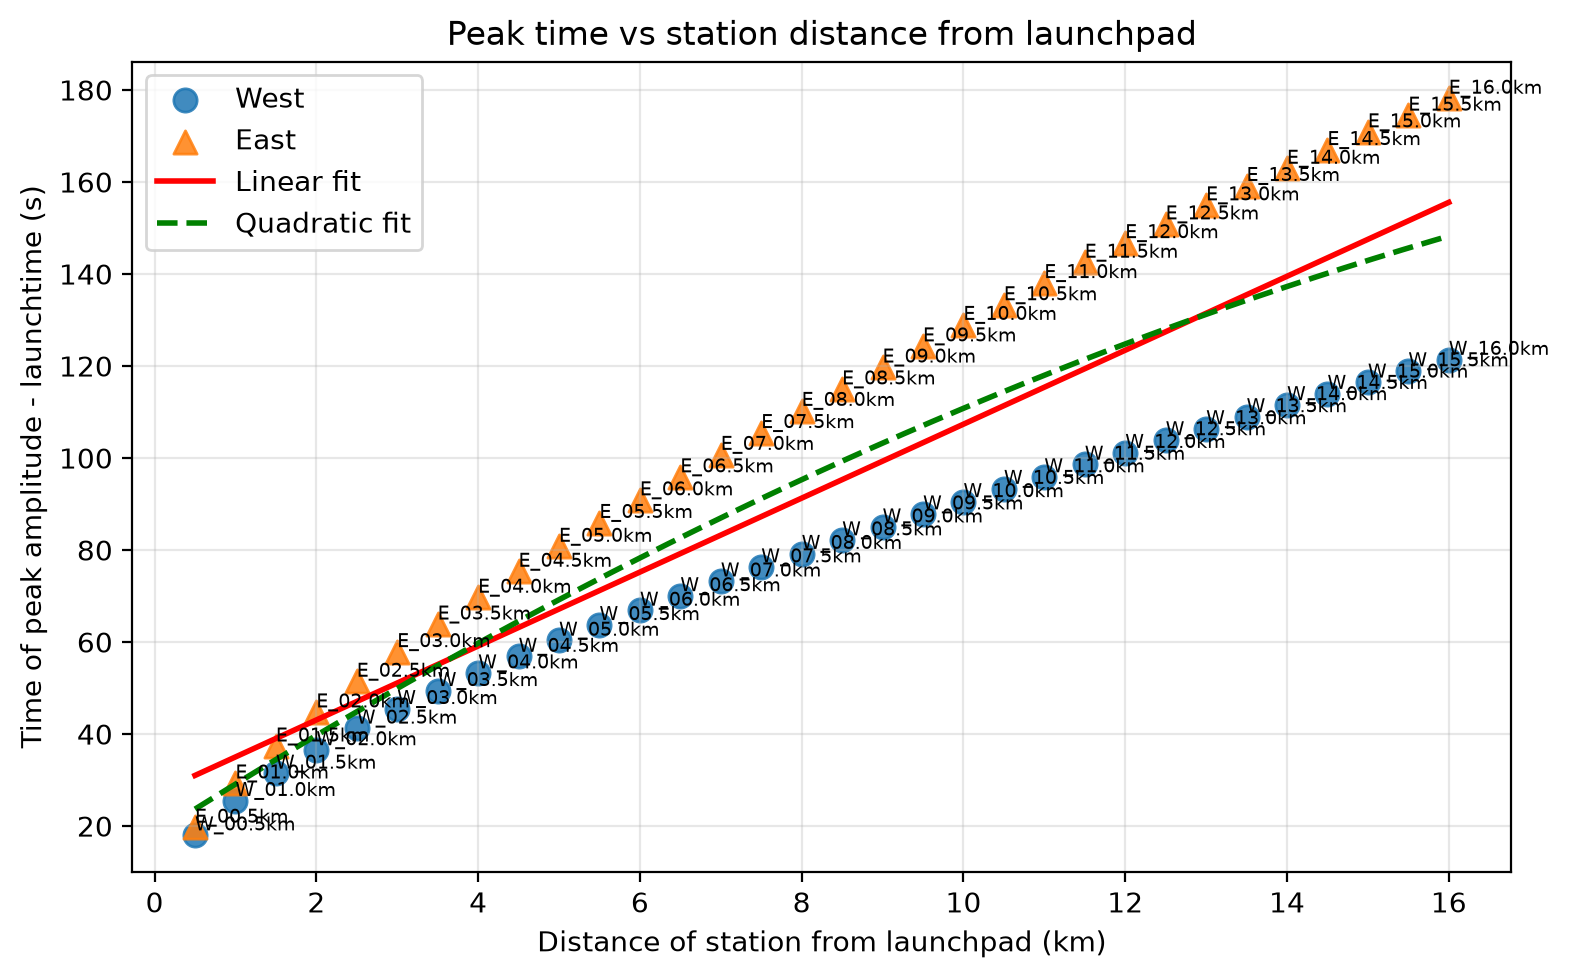
\includegraphics[width=\textwidth]{figures/synthetic_peaktime_vs_distance}
  \caption{Synthetic peak arrival time versus station distance from
    SLC-39B. East stations (triangles) show systematically later
    arrivals than west stations (circles) at the same distance.
    The solid red line is the linear fit
    $t = 29.6 + 8.0\,r$~s ($r$ in km, apparent speed 125~m~s$^{-1}$);
    the dashed green line is the quadratic fit.}
  \label{fig:synthetics}
\end{figure}

\begin{equation}
  t = 29.57 + 8.00\,R
  \label{eq:tsyn}
\end{equation}
($t$ in s, $R$ in km), an apparent propagation speed of
$\sim$125~m~s$^{-1}$. This is close to the 136~m~s$^{-1}$ derived from
the observations (Equation~\ref{eq:tlin}), so the forward model
reproduces the observed slowness without any adjustment. The slowness
comes entirely from source motion and directivity, not from a slow
propagation medium. The combined fit hides a large azimuthal
difference: fitted separately, the west line gives 6.2~s~km$^{-1}$
($\sim$162~m~s$^{-1}$) and the east line 9.8~s~km$^{-1}$
($\sim$102~m~s$^{-1}$). The synthetic intercept (29.6~s) is much
larger than the observed one (5.3~s), and the synthetic fit spans
0.5--16~km compared with $\lesssim$8~km for the real network. A
like-for-like comparison at the actual station coordinates is made in
Section~\ref{sec:model_data}.


%% ============================================================
\section{Model--Data Comparison}
\label{sec:model_data}

\subsection{Timing Comparison}
\todo{Compare slope and intercept of model vs.\ observed arrival-time
fits. Intercept mismatch may indicate a source timing issue.}

\subsection{Amplitude Comparison}
\todo{Compare amplitude decay rate; discuss east--west asymmetry and
sensitivity to cone model parameters.}

\subsection{Interpretation}
\todo{What is controlled by trajectory, source strength, and
directivity?}


%% ============================================================
\section{Discussion}

\subsection{What Controls Infrasound Observations?}
\todo{Geometry, moving source, directional radiation, plume physics.}

\subsection{Limitations}

The principal simplifications of the forward model include the
assumption of a constant sound speed, neglect of atmospheric
stratification and wind refraction, and the use of a simplified
point-source representation. Future work could address these by
incorporating atmospheric ray-tracing or full-waveform propagation
modelling.

\subsection{Implications}
\todo{Rocket launches as controlled geophysical sources; relevance to
volcano infrasound and atmospheric acoustics.}


%% ============================================================
\section{Conclusions}

\todo{Write prose conclusions. Key points from outline:}
\begin{itemize}
  \item The dense array enables new quantitative insights into
    near-field seismo-acoustic signals from a super-heavy launch
    vehicle.
  \item A single, well-instrumented launch yields greater insight into
    source characteristics and propagation than a large number of
    sparsely recorded events.
  \item The observed amplitude decay and apparent propagation speed are
    inconsistent with a stationary, isotropic source; a directional,
    moving source model is essential for interpretation.
  \item The combined seismo-acoustic dataset provides a framework for
    future studies of both individual launches and the multi-year KSC
    launch record.
\end{itemize}


%% ============================================================
\section*{Data and Code Availability}

Waveform data will be archived through EarthScope upon publication.
Analysis code is available at
\textcolor{orange}{\texttt{https://github.com/[USERNAME]/KSCRocketSeismoHydrology}} \todo{replace with actual URL}.

\begin{acknowledgements}
The SmartSolo instruments were provided by the EarthScope Primary
Instrument Center (EPIC). Gem infrasound nodes were provided by Boise
State University. \todo{Complete acknowledgements: Katherine, Don?,
Robert, John?, others? NASA MSFC. Any grants to acknowledge?}
\end{acknowledgements}

\section*{Author Contributions}

\todo{Complete CRediT author contributions statement.}

%% ============================================================
%% Bibliography style is set by seismica.cls (abbrvnat_seismica_upcasetitle.bst)
\bibliography{artemis2}  %% references go in artemis2.bib

%% ---- Placeholder bibliography until .bib file is built ----
%% Remove the two lines above and uncomment the block below
%% to use a manual list while the .bib file is being assembled.
%
% \begin{thebibliography}{9}
% \bibitem{Beyreuther2010}
%   Beyreuther, M., Barsch, R., Krischer, L., Megies, T., Behr, Y., \& Wassermann, J. (2010).
%   ObsPy: A Python Toolbox for Seismology.
%   \textit{Seismological Research Letters}, 81(3), 530--533.
%   \url{https://doi.org/10.1785/gssrl.81.3.530}
% \end{thebibliography}

\end{document}
